%=== CHAPTER FOUR (4) ===
%=== Test and Experiments ===

\chapter{Test and Experiments}

\section{Datasets}

Evaluation are performed in several datasets including KITTI stereo 2015 dataset\cite{Menze2015CVPR},  Oxford RobotCar dataset\cite{maddern20171} and NTU dataset collected in NTU. The listing of used datasets is shown in Table \ref{tbl:datasetsinfo}


\begin{table*}
	\centering
	\caption{Information of datasets used }
	\begin{tabular}{|c|c|c|c|}
		\hline
		Datasets & Settings & Approx Scale & Diversity \\
		\hline
		KITTI &  rural area & $<$ 1 hour & one city, one weather condition, daytime \\
		\hline
		Oxford &  city & 214 hours & one city, multiple weather conditions, daytime \\
		\hline
		NTU &  campus & $<$ 1 hour & one campus (NTU), one weather condition \\
		\hline
	\end{tabular}
	\label{tbl:datasetsinfo}
\end{table*}

\subsection{KITTI Visual Odometry Dataset}

KITTI Visual Odometry 2012 is a part of KITTI Vision Benchmarck Suite, presented in \cite{Geiger2012CVPR,Menze2015CVPR}. KITTI datasets are captured by driving around a mid-size city, in rural areas and on highways. The recording platform is equipped with two high resolution stereo camera systems, capturing color and gray images, a Velodyne HDL-64E LIDAR, and an OXTS RT 3003 localization system which combines GPS, GLONASS, an IMU and RTK correction signals.

KITTI Visual Odometry Evaluation 2012 provides 11 sequences with ground truth trajectories for training, and another 11 sequences without ground truth for evaluation. Example images are shown in Figure \ref{fig:kittiexamples}. In order to evaluate CORB-SLAM system, sequence 00 is utilized and separated into two sub sequences with proper length of overlap. The following separating method is employed: We assume the time period of a KITTI sequence if $Seq.[0,t]$. Then the sequence is separated into two sub sequences $Seq.[0,\frac{t}{2}+\delta{t}]$ and $Seq.[\frac{t}{2},t]$ as the assumed input of two client robots. 

\begin{figure}[H]
	\centering
	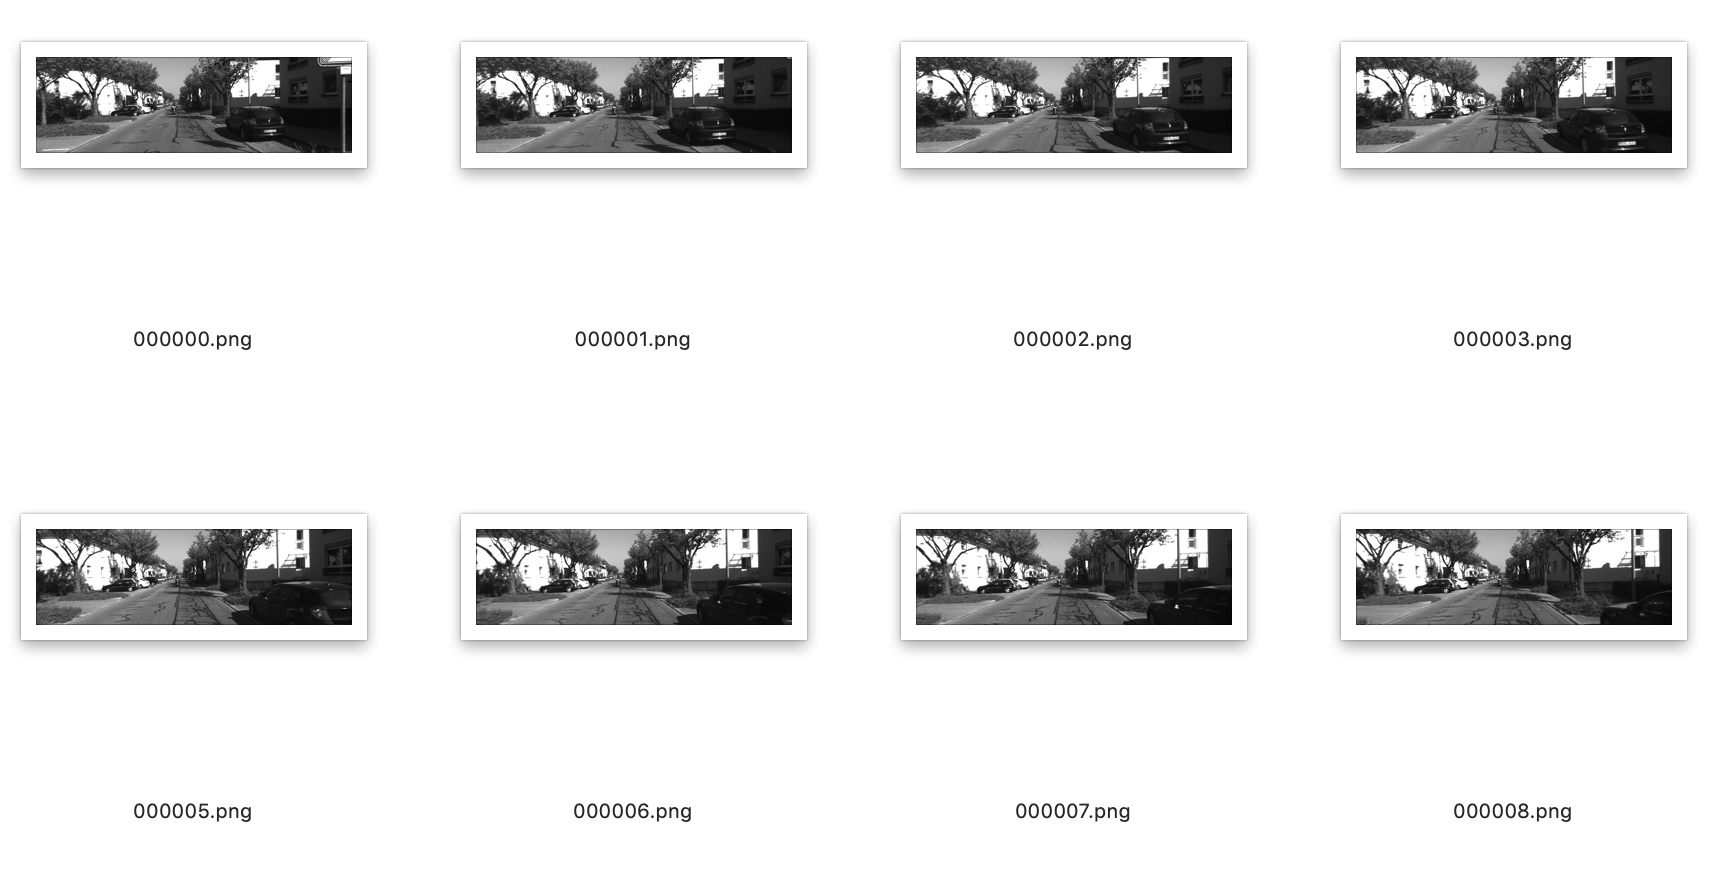
\includegraphics[width=5in]{Chapter4/kittiexamples.eps}
	\caption{Example image in KITTI Visual Odometry 2012 dataset.}
	\label{fig:kittiexamples} 
\end{figure}

\subsection{Oxford RobotCar Dataset}
Oxford RobotCar Dataset is presented by Will Maddern et al. in \cite{maddern20171}, as a challenging dataset for autonomous driving. Collected over the period of May 2014 to December 2015, this datasets recorded images from 6 cameras mounted Nissan LEAF, along with LIDAR, GPS and INS ground truth. Images were recorded under different weather and illumination condition  from 9:00 to 16:00 on average, from May to December. Example images is shown in Figure \ref{fig:robotcarexamples}.

\begin{figure}[H]
	\centering
	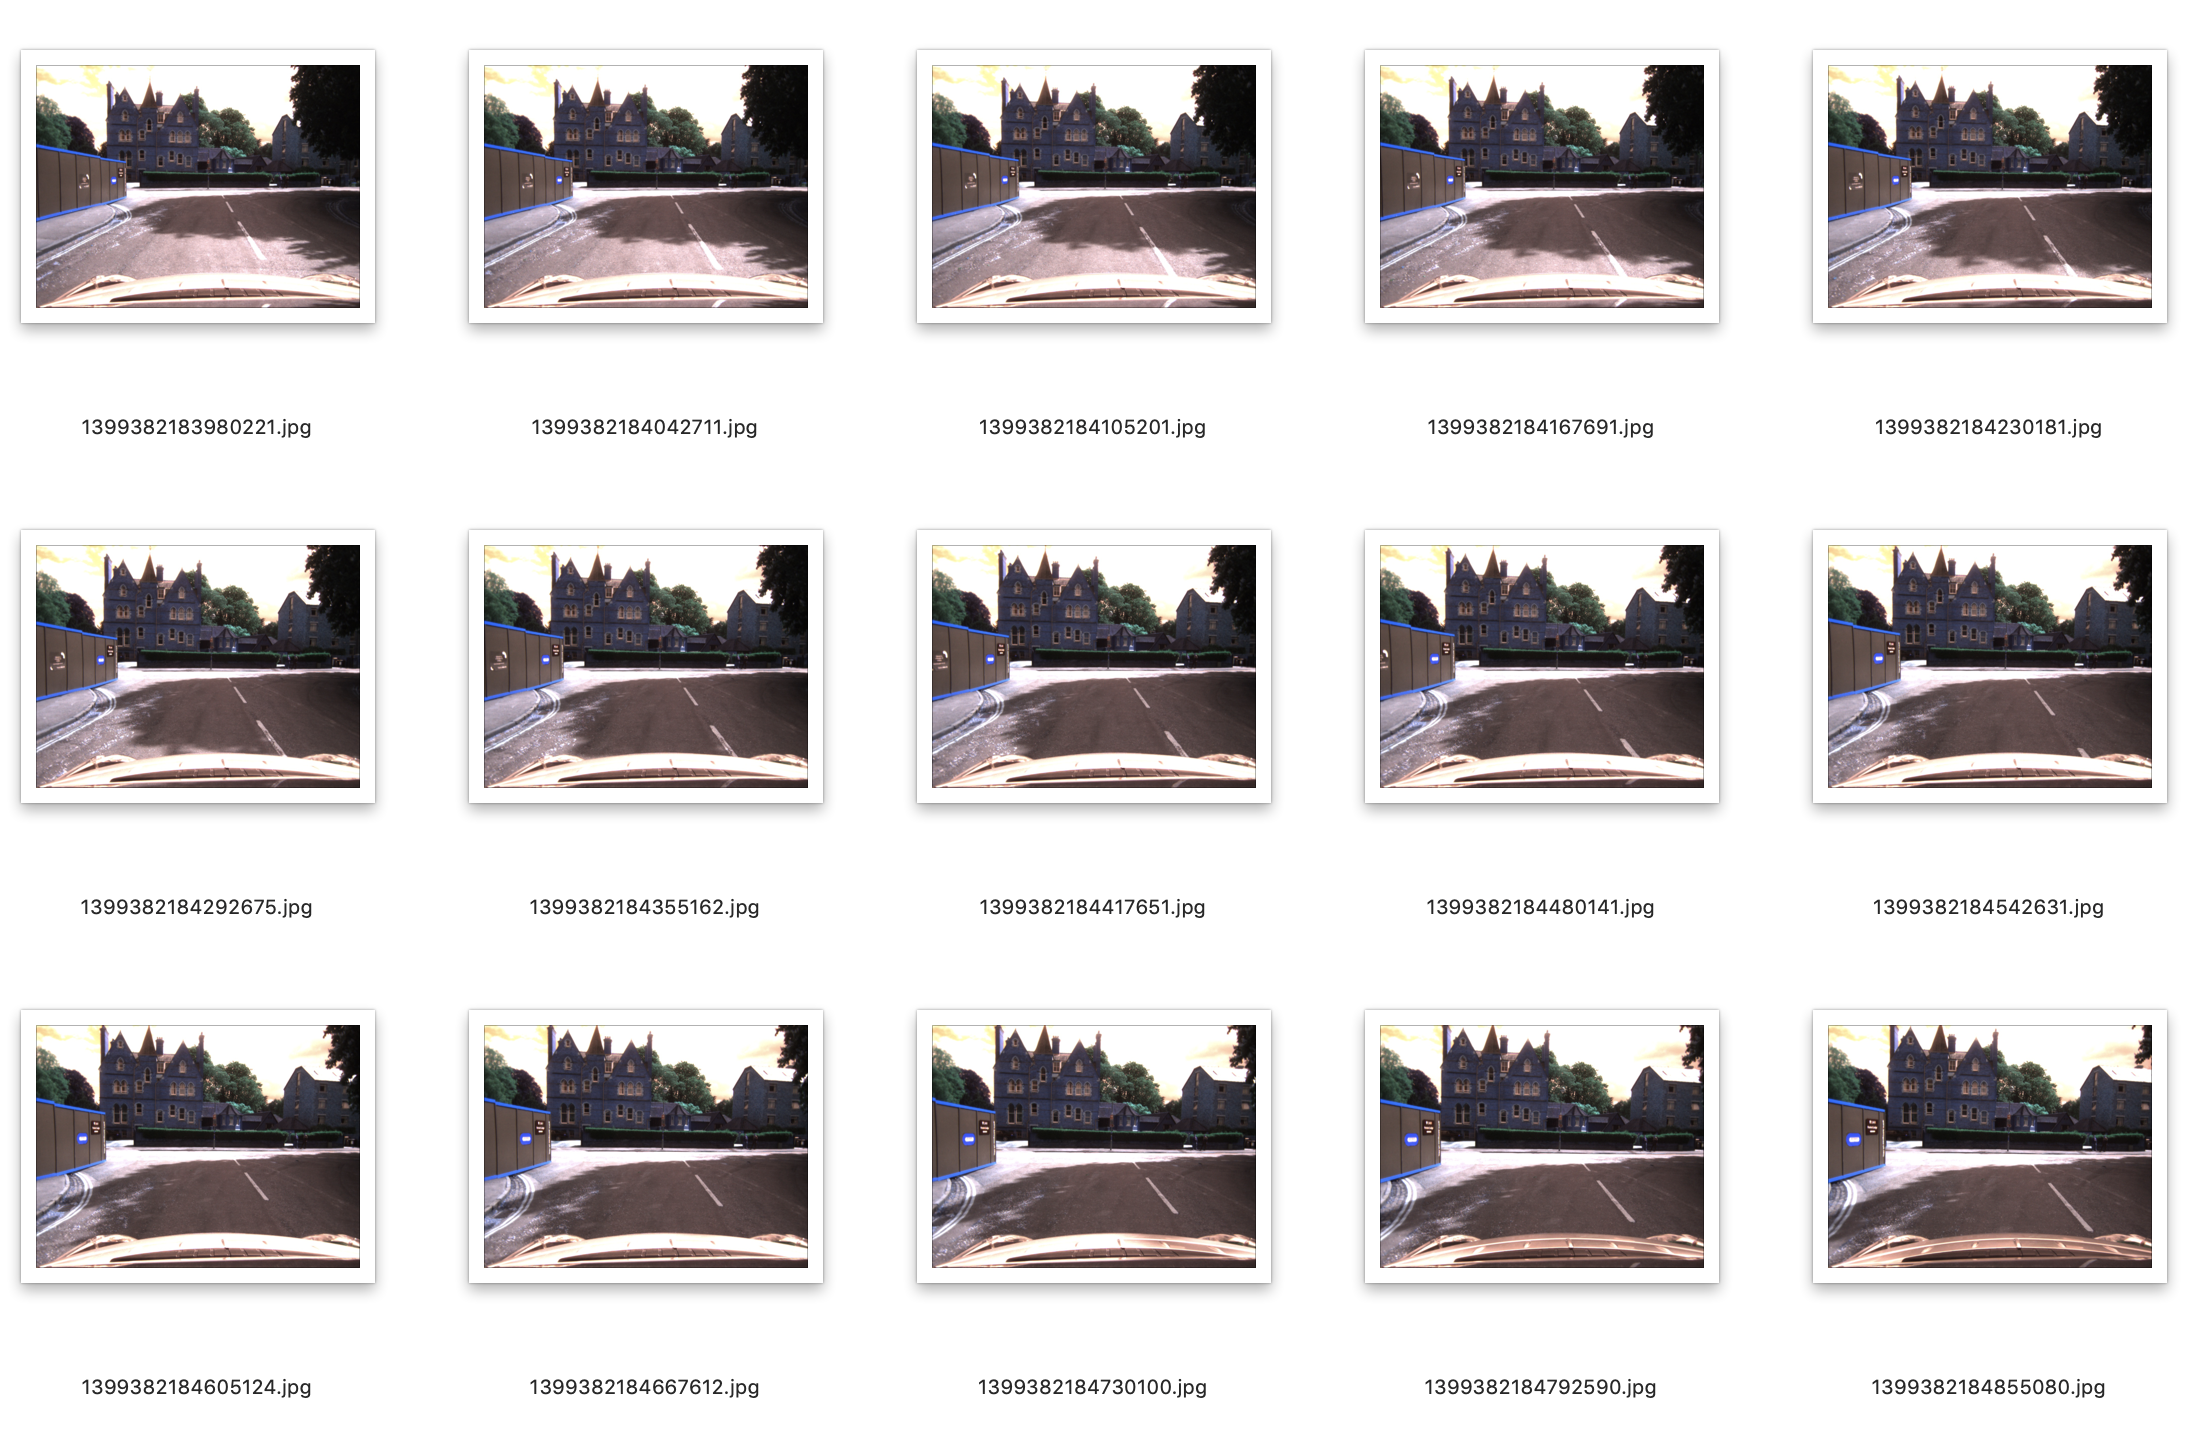
\includegraphics[width=5in]{Chapter4/robotcarexamples.eps}
	\caption{Example image in robotcar dataset.}
	\label{fig:robotcarexamples} 
\end{figure}

The RobotCar platform is a Nissan LEAF equipped with sensors as following \cite{maddern20171}:

\begin{enumerate}
	\item Stereo Camera: Bumblebee XB3 trinocular stereo camera $\times$ 1, 1/3'' Sony ICX445 CCD, 1280$\times$960$\times$3, 16Hz, 3.88mm lens, $66^{\circ}$ HFoV, 12/24cm baseline, global shutter.
	\item Monocular Camera: Grasshopper2 $\times$ 3, 2/3'' ICX285 CCD, 1024$\times$1024, 11.1Hz, 2.67mm fisheye lens, $180^{\circ}$, global shutter.
	\item 2D LIDARL SICK LMS-151 2D LIDAR $\times$ 2, $270^{\circ}$ FoV, 50Hz, 50m range, $0.5^{\circ}$ resolution.
	\item 3D LIDAR: SICK LD-MRS 3D LIDAR $\times$ 1, $85^{\circ}$ HFoC, $3.2^{\circ}$ VFoV, 4 panes, 12.5Hz, 50m range, $0.125^{\circ}$ resolution.
	\item GPS/INS Module: NovAtel SPAN-CPT ALIGN inertial and GPS navigation system $\times$ 1, 6 axis, 50Hz, GPS/GLONASS, dual antenna.
 \end{enumerate}

The RobotCar platform and the sensor locations are demonstrated in Figure \ref{fig:robotcarsensorlocation}.

\begin{figure}[H]
	\centering
	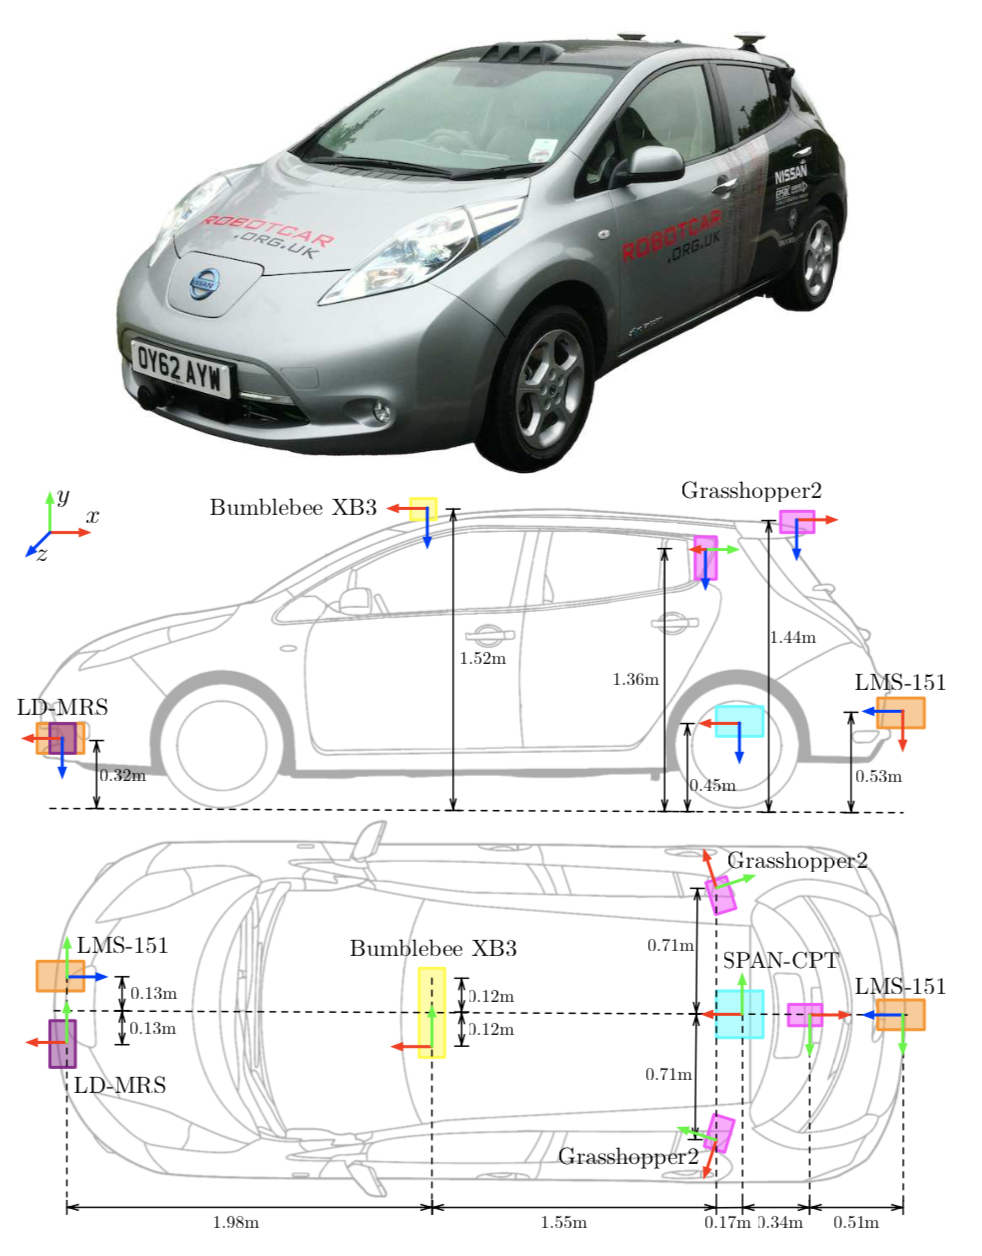
\includegraphics[width=5in]{Chapter4/robotcarsensorlocation.eps}
	\caption{The robotcar platform and sensor location diagram.}
	\label{fig:robotcarsensorlocation} 
\end{figure}

RobotCar dataset is especially suitable to evaluate life-long SLAM systems, since it contains images taken in different hours of daytime under different illumination conditions, and in different seasons. The comparison between image in different illumination conditions and different seasons is shown in Figure \ref{fig:robotcarcomparisonillu} and \ref{fig:robotcarcomparisonseason}.

Because the dataset was collected in real-world outdoor street environment, there are some frames with overexposure demonstrated in Figure \ref{fig:robotcaroverexposed}, which cannot be process by vSLAM. Therefore, in this work, this dataset is intercepted into two sub sequences excluding overexposed images.

The sub sequences selected is listed in Table \ref{tbl:robotcarpartial}. The ground truth GPS/INS trajectories of two sub sequences are shown in Figure \ref{fig:robotcargt}. The ground truth trajectories of two sub sequences are combined in Figure \ref{fig:robotcaroverallgt}.

\begin{figure}[H]
	\centering
	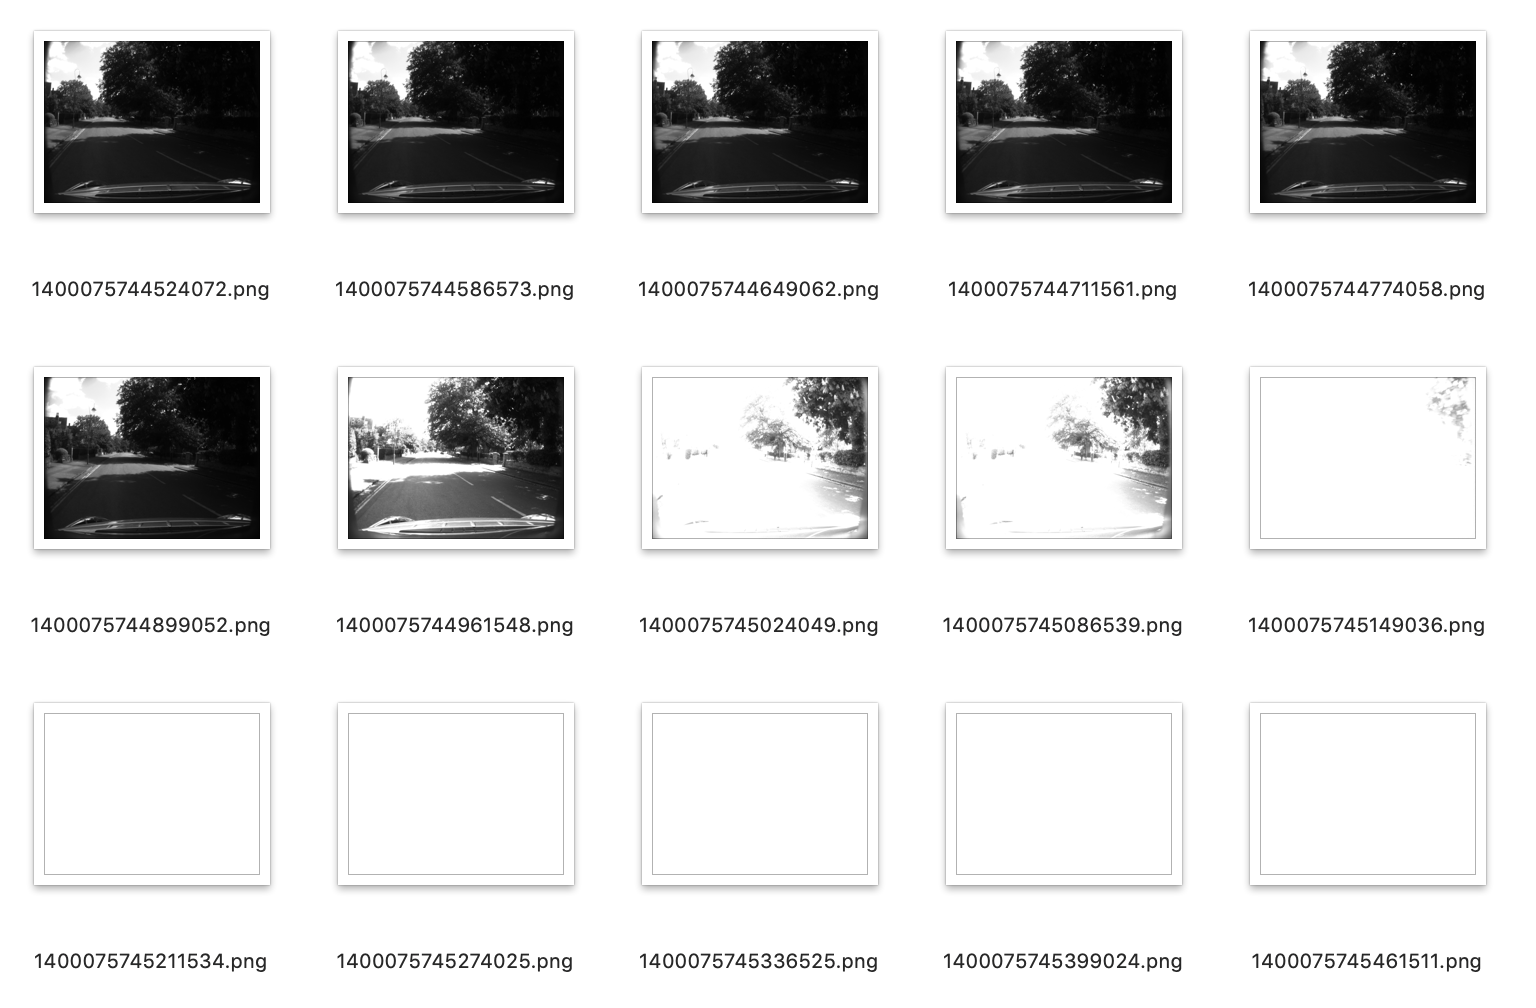
\includegraphics[width=5in]{Chapter4/robotcaroverexposed.eps}
	\caption{Image sequence with overexposed frames in RobotCar dataset.}
	\label{fig:robotcaroverexposed} 
\end{figure}

\begin{table*}
	\centering
	\caption{Partial datasets selected in RobotCar dataset.}
	\begin{tabular}{|c|c|c|c|c|}
		\hline
		Seq. No. & Data(M/D/Y) & Time & Weather & Timestamps  \\
		\hline
		0&07/14/2014&14:49&\tabincell{c}{summer\\overcast}& \tabincell{c}{1405349847738682 to\\1405350059147905}\\
		\hline
		1&12/05/2014&15:42&\tabincell{c}{winter\\overcast}& \tabincell{c}{1417794166325288 to\\1417794407042717}\\
		\hline
	\end{tabular}
	\label{tbl:robotcarpartial}
\end{table*}

\begin{figure}
	\centering
	\subfigure[Ground truth trajectory of Seq.0.]{
		\begin{minipage}[t]{0.4\linewidth}
			\centering
			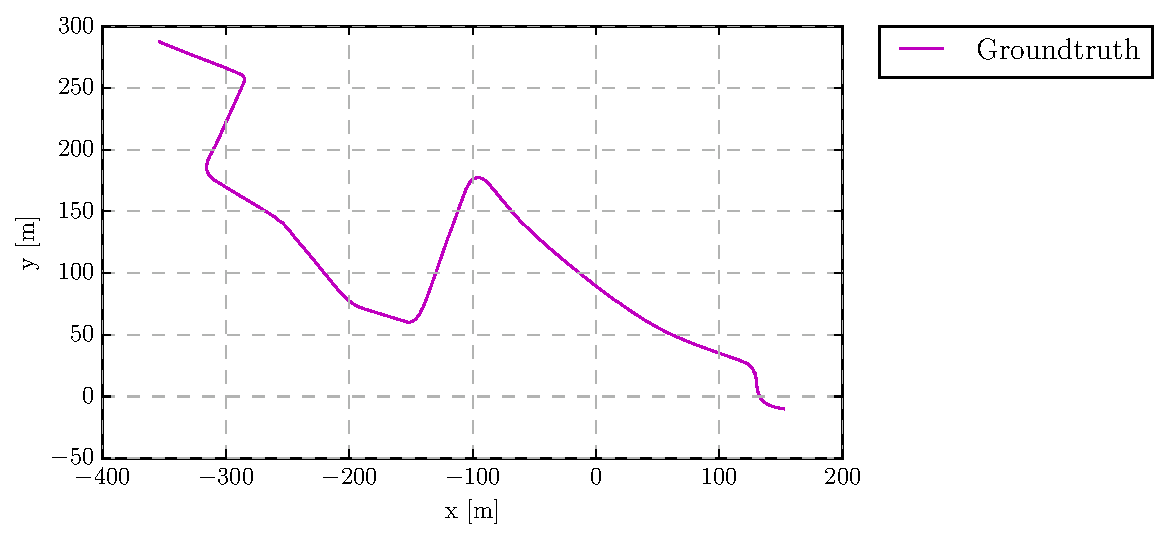
\includegraphics[width=2in]{Chapter3/0714gt.pdf}
		\end{minipage}
	}
	\subfigure[Ground truth trajectory of Seq.1.]{
		\begin{minipage}[t]{0.4\linewidth}
			\centering
			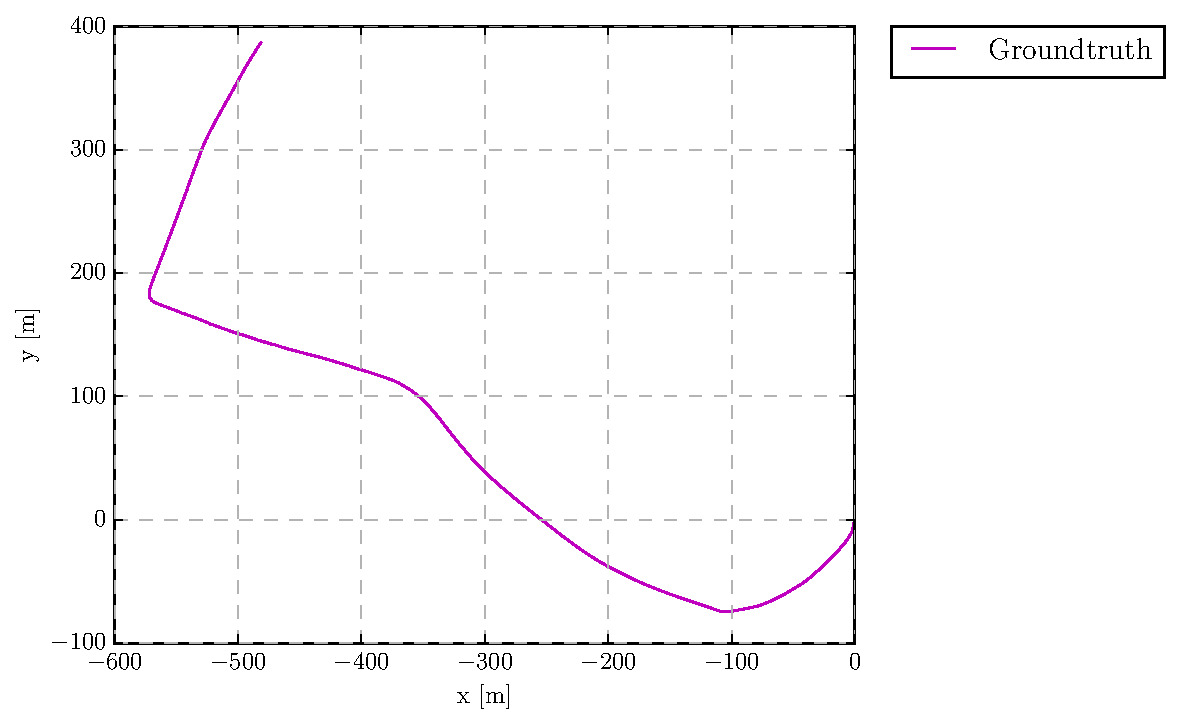
\includegraphics[width=2in]{Chapter3/1205gt.pdf}
		\end{minipage}
	}
	\caption{Ground truth trajectories of two sub sequences.}
	\label{fig:robotcargt}
\end{figure}

\begin{figure}[H]
	\centering
	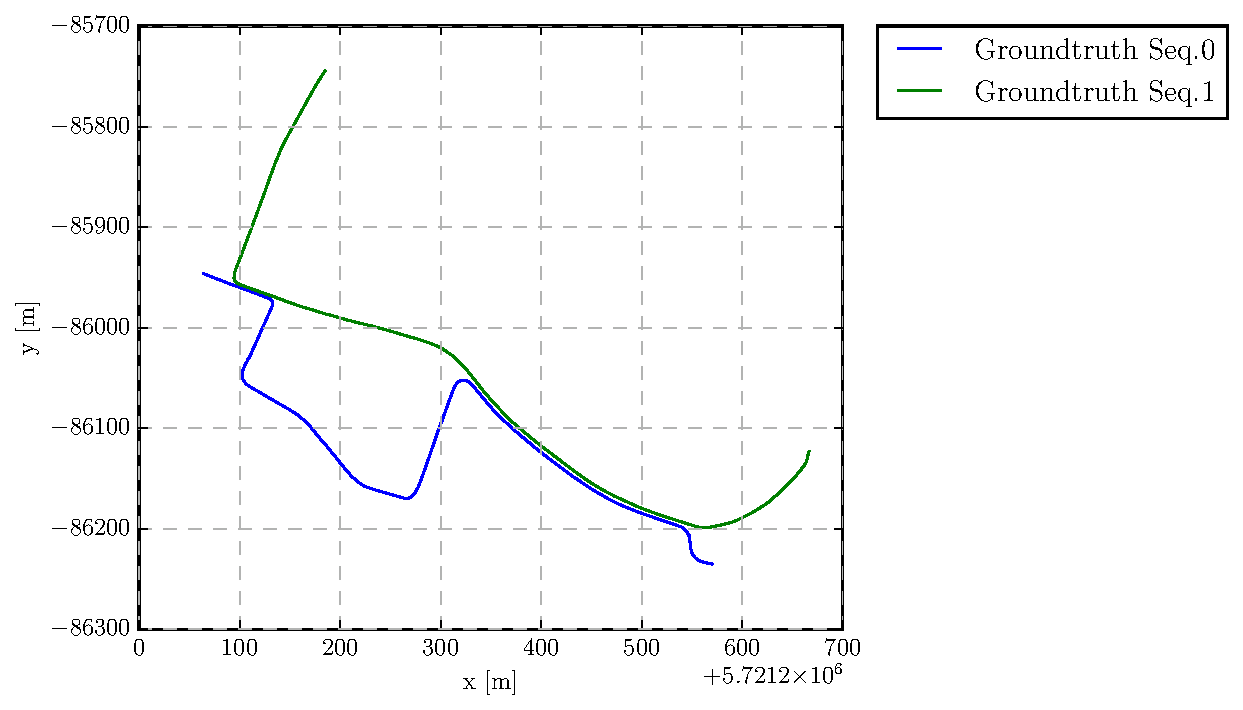
\includegraphics[width=5in]{Chapter3/overall_gt_top_.pdf}
	\caption{Overall ground truth trajectory of Seq.0 and Seq.1.}
	\label{fig:robotcaroverallgt} 
\end{figure}

\begin{figure}
	\centering
	\subfigure[pic1.]{
		\begin{minipage}[t]{0.4\linewidth}
			\centering
			
\includegraphics[width=2in]{thereisafigure.eps}
			%\caption{fig1}
		\end{minipage}
	}
	\subfigure[pic2.]{
		\begin{minipage}[t]{0.4\linewidth}
			\centering
			
\includegraphics[width=2in]{thereisafigure.eps}
			%\caption{fig2}
		\end{minipage}
	}
	\caption{Comparison of images in different seasons in RobotCar dataset.}
	\label{fig:robotcarcomparisonseason}
\end{figure}

\begin{figure}
	\centering
	\subfigure[pic1.]{
		\begin{minipage}[t]{0.4\linewidth}
			\centering
			
\includegraphics[width=2in]{thereisafigure.eps}
			%\caption{fig1}
		\end{minipage}
	}
	\subfigure[pic2.]{
		\begin{minipage}[t]{0.4\linewidth}
			\centering
			
\includegraphics[width=2in]{thereisafigure.eps}
			%\caption{fig2}
		\end{minipage}
	}
	\caption{Comparison of images in different illumination in RobotCar dataset.}
	\label{fig:robotcarcomparisonillu}
\end{figure}
	
\subsection{NTU Dataset}

Our NTU dataset is collected on a husky UGV platform, recording driving around the carpark in front of School of EEE.

Our platform is a HUSKY Clearpath robot, equipped with a ZED stereo camera $\times$ 1, 672$\times$376, $87^{\circ}$ HFoV, $56^{\circ}$ VFoV. The picture of the platform and example images are shown in Figure \ref{fig:ntuplatform} and \ref{fig:ntuexamples}.

\begin{figure}[H]
	\centering
	
\includegraphics[width=5in]{thereisafigure.eps}
	\caption{Overview picture of NTU Husky platform.}
	\label{fig:ntuplatform} 
\end{figure}

\begin{figure}[H]
	\centering
	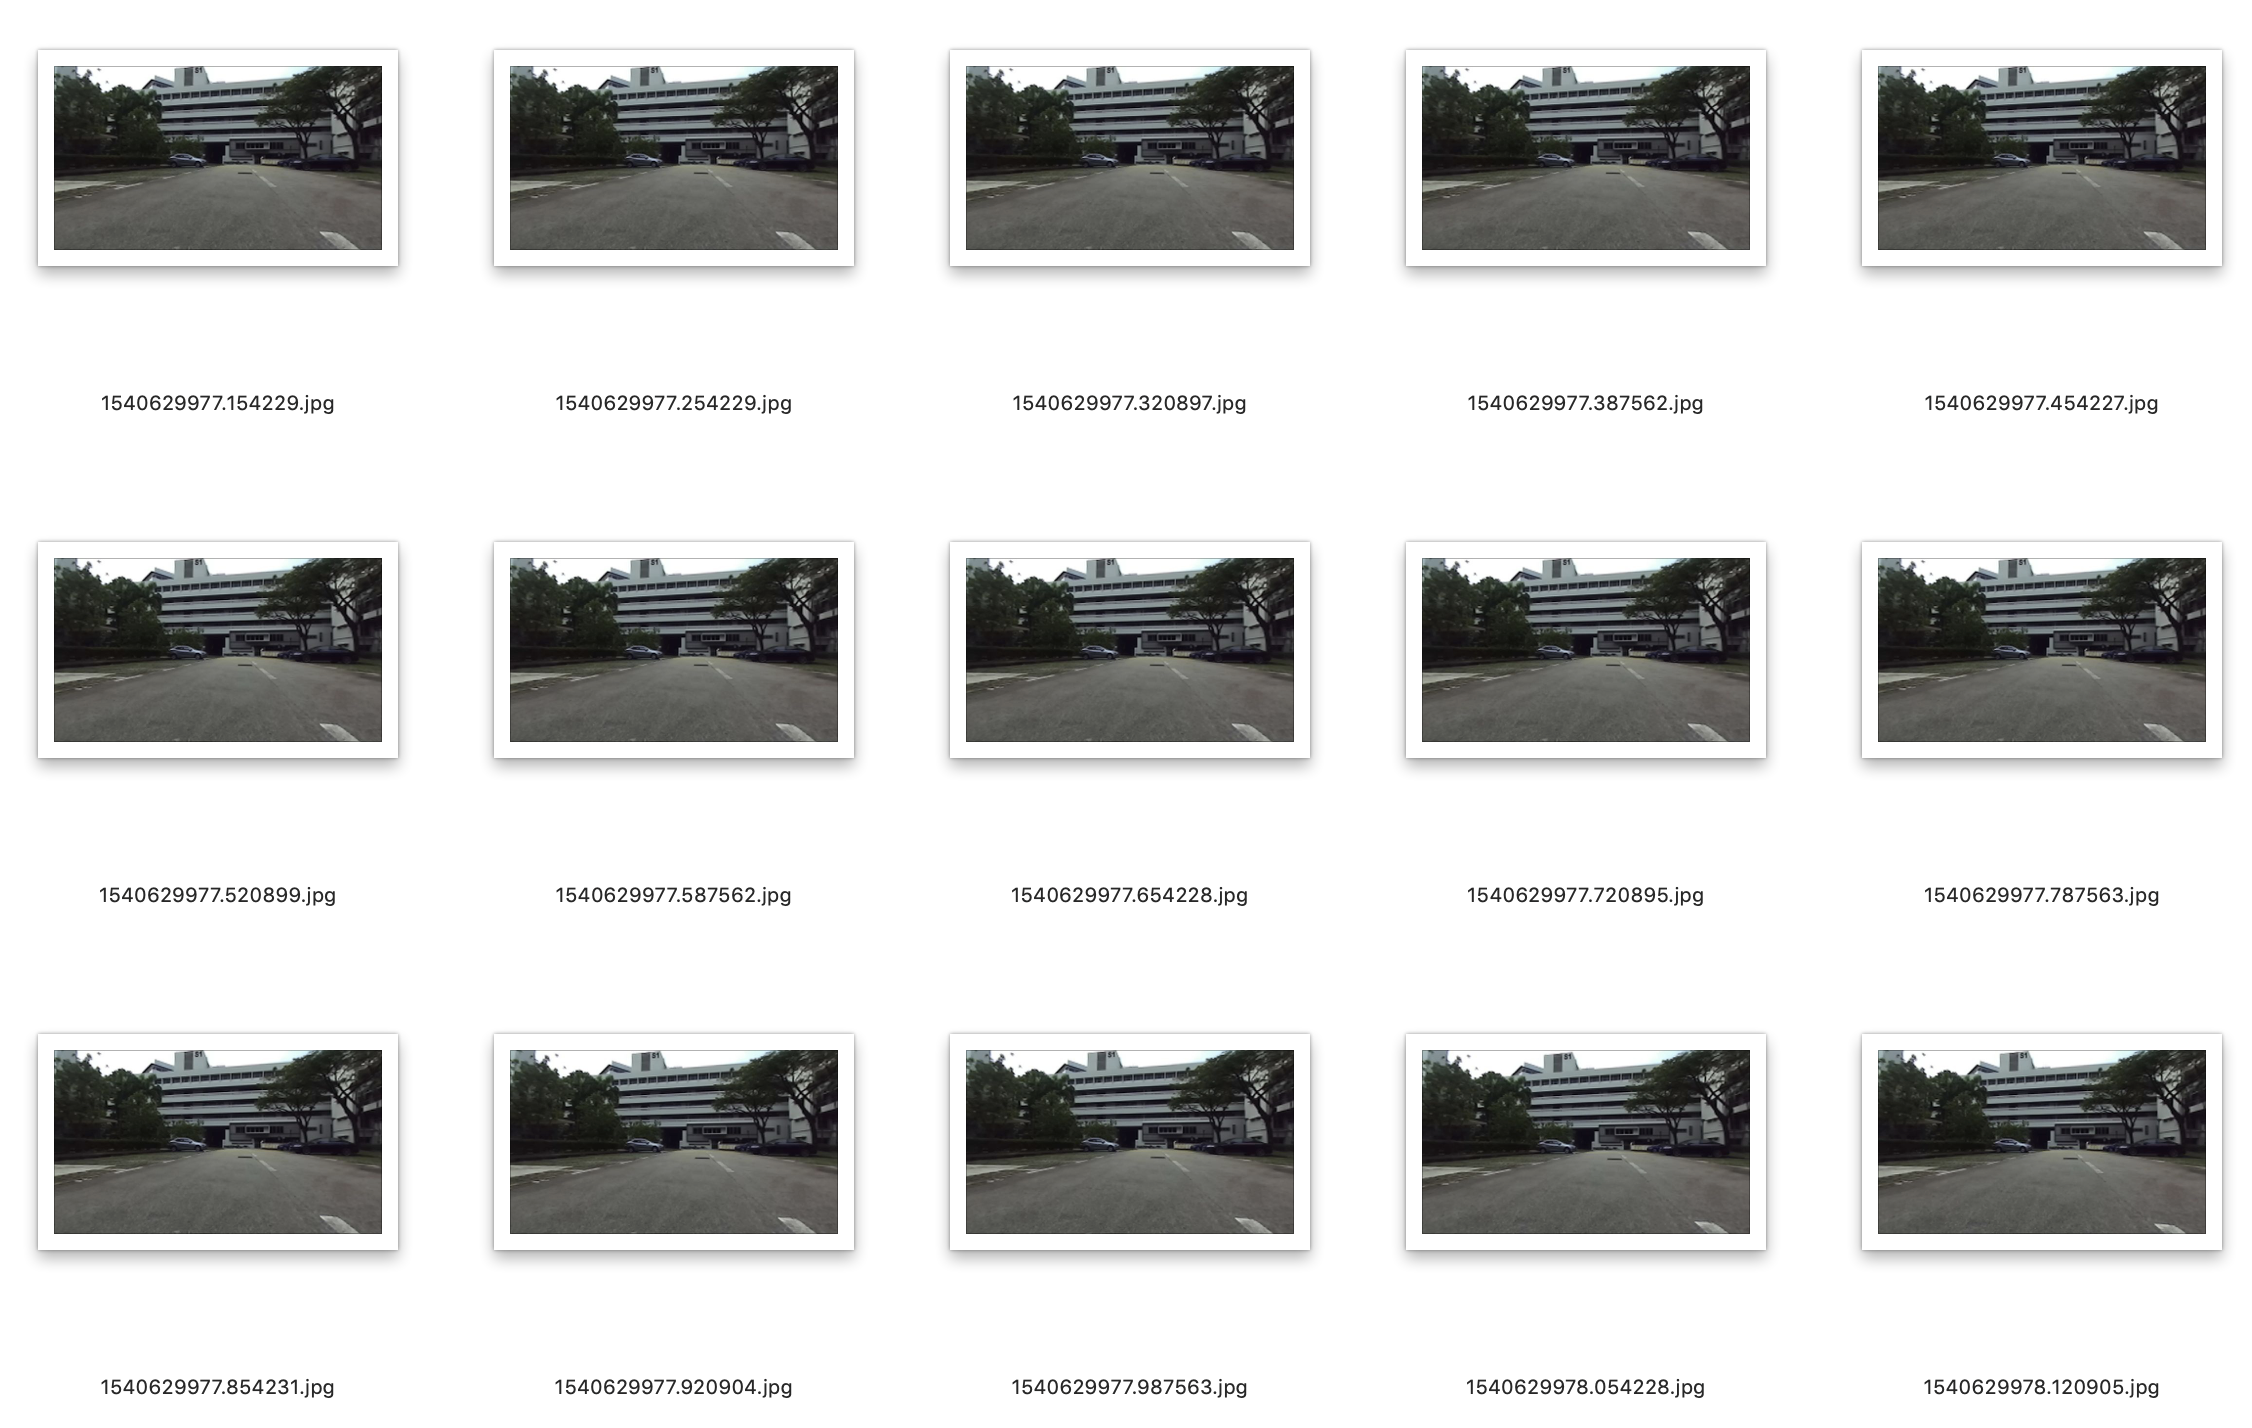
\includegraphics[width=5in]{Chapter4/ntuexamples.eps}
	\caption{Example images of NTU dataset.}
	\label{fig:ntuexamples} 
\end{figure}

\section{Evaluation of CORBSLAM}
\subsection{Evaluation on multi ground robots}
\subsection{Evaluation on multi hybrid robots}

\section{Evaluation under different illumination}


%=== END OF CHAPTER FOUR ===
\newpage
